\documentclass[12pt]{article}

\usepackage{fullpage}
\usepackage{graphicx, rotating, booktabs} 
\usepackage{times} 
\usepackage{natbib} 
\usepackage{indentfirst} 
\usepackage{setspace}
\usepackage{grffile} 
\usepackage{hyperref}
\usepackage{adjustbox}
\setcitestyle{aysep{}}


\singlespace
\title{
\textbf{Appendix: Reassessing the Public Goods Theory of Alliances}
	}

\bibliographystyle{apsr}

\begin{document}

\maketitle 

\doublespace

This appendix contains supporting materials for the test of Hypothesis 1 in ``Reassessing the Public Goods Theory of Alliances.'' 
Section 1 provides more detail about the variables in the model and Section 2 assesses model fit and accuracy. 
The final section summarizes a test that uses average economic weight in their alliances to predict percentage changes in military spending. 


\section{Variables} 


Olson and Zeckhauser use GDP to measure state size, so I constructed a measure of GDP using data from the Maddison Project, which provides longer historical coverage \citep{Boltetal2018}. 
I then take the natural log of GDP to address the variable's skewed distribution. 
I use military spending data from the Correlates of War Project \citep{SingerCINC1988}.  
All alliance membership data comes from Version 4 of the Alliance Treaty Obligations and Provisions (ATOP) data \citep{Leedsetal2002}.  


The dependent variable is percentage changes in military spending. 
Olson and Zeckhauser use defense spending as a share of GDP as their dependent variable, which is the source of previously described identification problems \citep{Kronmal1993, PluemperNeumayer2015}. 
I use percentage changes instead of the defense burden because this measure gives a sense of burdens from changing defense budgets with a lower risk of spurious inferences. 
Annual percentage changes in spending is the change in military spending as a share of the previous year's budget:


\begin{equation}
\mbox{\% Change Military Spending} = \frac{\mbox{Mil. Ex.}_t - \mbox{Mil. Ex.}_{t-1} }{ \mbox{Mil. Ex.}_{t-1} } = \frac{\Delta \mbox{Mil. Ex.} }{ \mbox{Mil. Ex.}_{t-1} }
\end{equation} 


Measuring percentage changes in spending matches Olson and Zeckhauser's emphasis on how alliance participants allocate resources to the military.
Positive percentage changes in spending imply an expanding defense budget and higher defense burden, all else equal.
Moreover, using percentage changes in spending mitigates the risk of spurious inferences due to non-stationarity in panel data. 
The log-level of military spending is not mean-reverting in long panels.
A differenced military spending variable has increasing variance over time, as budgets expand and generate larger changes. 
Modeling the DV in levels or changes might lead to spurious inferences \citep{GrangerNewbold1974}. 


Using percentage changes in military spending as the dependent variable benchmarks changes to budget size. 
This facilitates comparisons across states and years. 
A 2\% change is an equally burdensome increase in the defense budget for large and small states, all else equal. 


Besides the economic weight values in \textbf{Z}, I controlled for other variables that are correlated with alliance participation and military spending. 
I adjusted for international war \citep{Reiteretal2016}, civil war participation \citep{SarkeesWayman2010}, and a count of annual MIDs \citep{Gibleretal2016}. 
I also included measures of regime type, external threat \citep{LeedsSavun2007}, GDP, and the Cold War era. 

 


\section{Multilevel Model}

This section describes the priors on the multilevel model, convergence diagnostics for the Hamiltonian Monte Carlo, and results from running the same model with a weighted economic size in the alliance participation matrix. 


\subsection{Priors} 

All priors are specified to be weakly informative relative to the scale of the data \citep{Gelmanetal2017}. 
I summarize the prior distributions for each set of parameters in \autoref{tab:priors}. 
$p(\nu)$ is a well-behaved prior for the degrees of freedom in a t-distribution \citep{JuarezSteele2010}. 
Given that the median percentage change in military expenditures is 0.06, the priors are quite diffuse. 


\begin{table} % Create a table of priors.
\begin{center}
\begin{tabular}{c} 
$ p(\alpha) \sim N(0, 1)$  \\
$ p(\sigma) \sim \mbox{half-}N(0, 1) $ \\
$ p(\alpha^{yr}) \sim N(0, \sigma^{yr}) $ \\ 
$ p(\sigma^{yr}) \sim N(0, 1) $ \\
$ p(\alpha^{st}) \sim N(0, \sigma^{st}) $ \\ 
$ p(\sigma^{st}) \sim \mbox{half-}N(0, 1) $ \\ 
$ p(\gamma) \sim N(\theta, \sigma^{all}) $ \\ 
$ p(\theta) \sim N(0, .5) $ \\
$ p(\sigma^{all}) \sim \mbox{half-}N(0, 1) $ \\
$ p(\beta) \sim N(0, 1) $ \\
$ p(\nu) \sim gamma(2, 0.1)$ 
\end{tabular} 
\caption{Summary of Priors in Multilevel Model} 
\label{tab:priors}
\end{center} 
\end{table} 


To facilitate estimation, I use a non-centered parameterization for the state and year varying intercepts, as well as the $\gamma$ parameters \citep{BetancourtGirolani2015}. 
A non-centered parameterization decouples the mean and variance to express an equivalent prior, which makes sampling easier. 
I also employ a sparse matrix representation of the alliance membership matrix $\textbf{Z}$ to speed up estimation. 


\subsection{Convergence} 


There were no divergent iterations in sampling. 
However, there are other threats to inference from the posterior samples. 
Given heavy tails in percentage changes of military spending, STAN might have struggled to explore the posterior distribution. 


Energy plots can diagnose this problem. 
\autoref{fig:energy-plot} plots the marginal energy distribution and the first differenced distribution. 
If the two histograms do not overlap, sampling was impeded by heavy tails. 
The substantial overlap in the distributions for all four chains in \autoref{fig:energy-plot} indicates this was not a problem. 


\begin{figure}
	\centering
		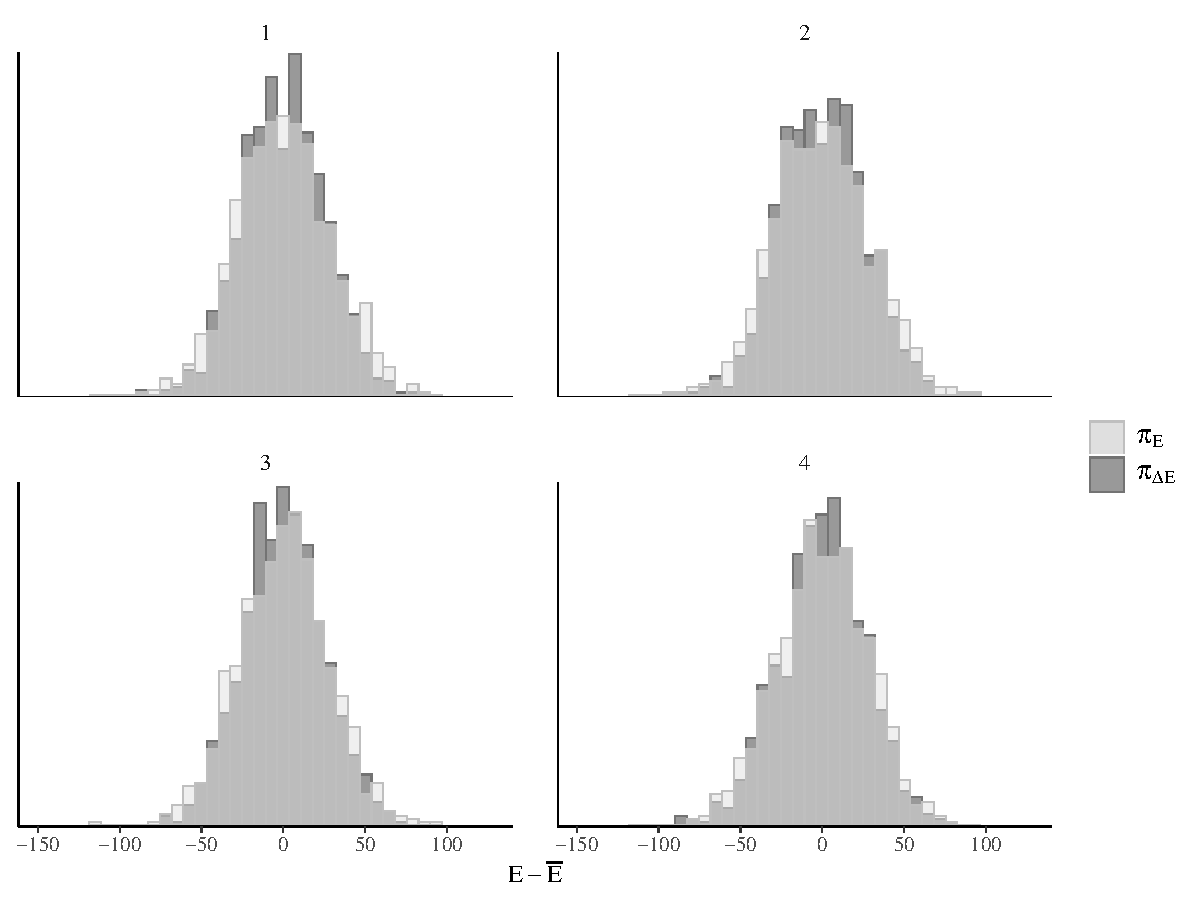
\includegraphics[width=0.55\textwidth]{energy-plot.pdf}
	\caption{Energy plot of multilevel model results. Greater overlap in the two histograms indicates adequate exploration of the posterior distribution. }
	\label{fig:energy-plot}
\end{figure}


The split $\hat{R}$ statistic is another way to assess convergence. 
$\hat{R}$ compares the behavior of each chain by measuring the ratio of the average variance of draws within each chain to the variance of the pooled draws across chains. 
When $\hat{R}$ is close to 1, all the chains have similar variance, and are therefore in equilibrium. 


The standard heuristic is that an $\hat{R}$ greater than 1.1 is problematic. 
\autoref{fig:rhat-plot} plots the $\hat{R}$ statistic for every parameter in the model. 
No parameters generate concern, even at a more conservative threshold of 1.05. 


\begin{figure}[htbp]
	\centering
		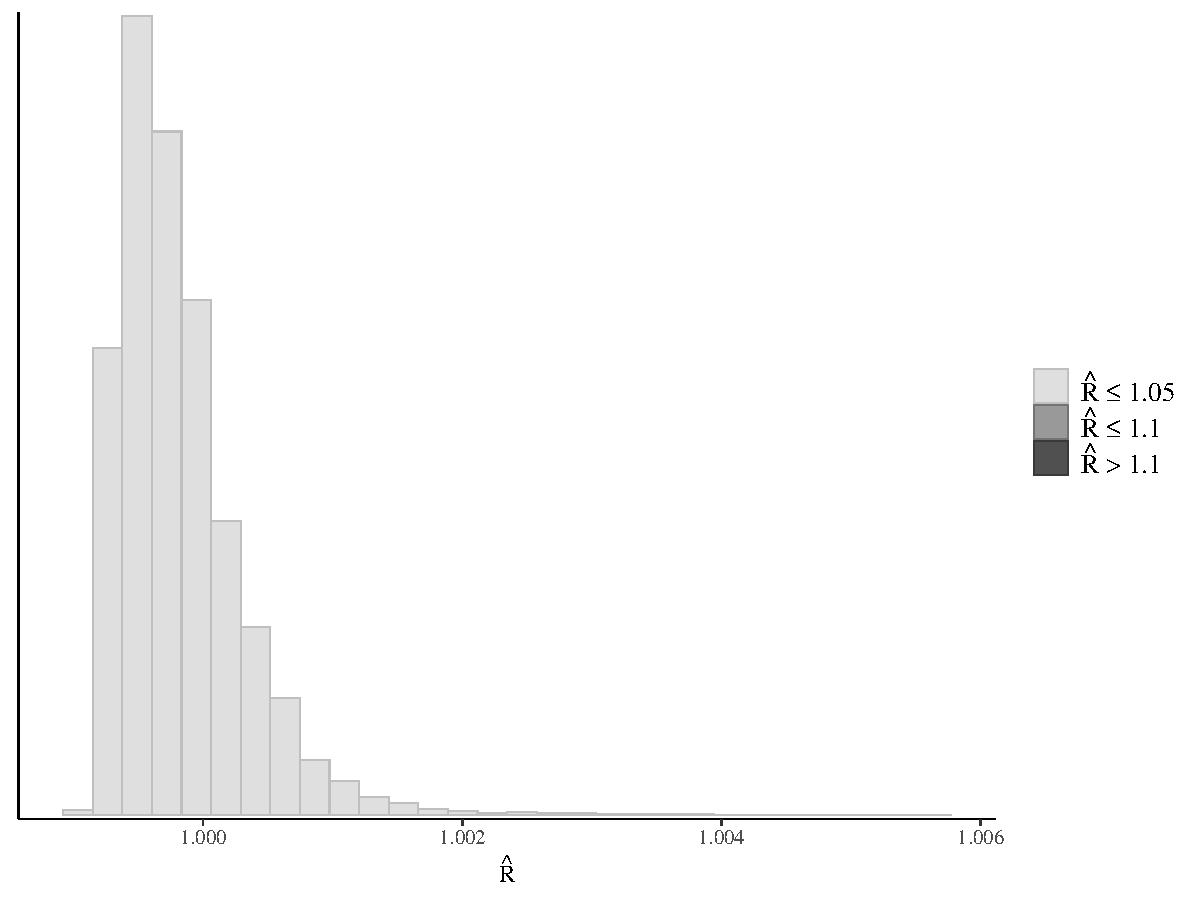
\includegraphics[width=0.55\textwidth]{rhat-plot.pdf}
	\caption{Histogram of split $\hat{R}$ statistic for all parameters in the multilevel model.}
	\label{fig:rhat-plot}
\end{figure}


\subsubsection{Inferences from Simulated Data}


To assess if the model gives reasonable answers, I simulated data and associated parameters, then re-estimated the model on the simulated data.
The model is a good fit if the credible intervals contain the known parameter values for the simulated data. 
This process checks whether the model can recover parameters from a known data-generating process that matches the model. 


I simulate a hypothetical dataset with 2000 observations of 50 states observed over 200 years.
I used part of the observed alliance data from the paper, due to problems simulating an alliance membership matrix with the same characteristics as the alliance data. 
There are 100 alliances in this data, and 2 state-level control variables. 
The hypothetical outcome is drawn from a Cauchy distribution with mean 0 and a scale of .25, which is more heavy-tailed than even my observed data. 


I then simulate 2,000 draws of the outcome using the generated quantities block in STAN. 
The next step is selecting one of those draws of the outcome--- which includes the value of the outcome for each observation and the associated parameter values. 
I select the 12th draw from the posterior and check whether after estimating the model on these data, the credible intervals include zero. 


I focus on inferences about the $\gamma$, $\theta$ and $\sigma_{all}$ parameters, because all three affect my test of the public goods argument. 
As \autoref{fig:theta-sim-res} and \autoref{fig:sall-sim-res} show, the posteriors accurately capture the known values of the hyper-parameters $\theta$ and $\sigma_{all}$. 
In these figures, the true parameter value is marked with a thick black line, while the light gray shaded area shows the 90\% credible interval. 


\begin{figure}[htbp]
	\centering
		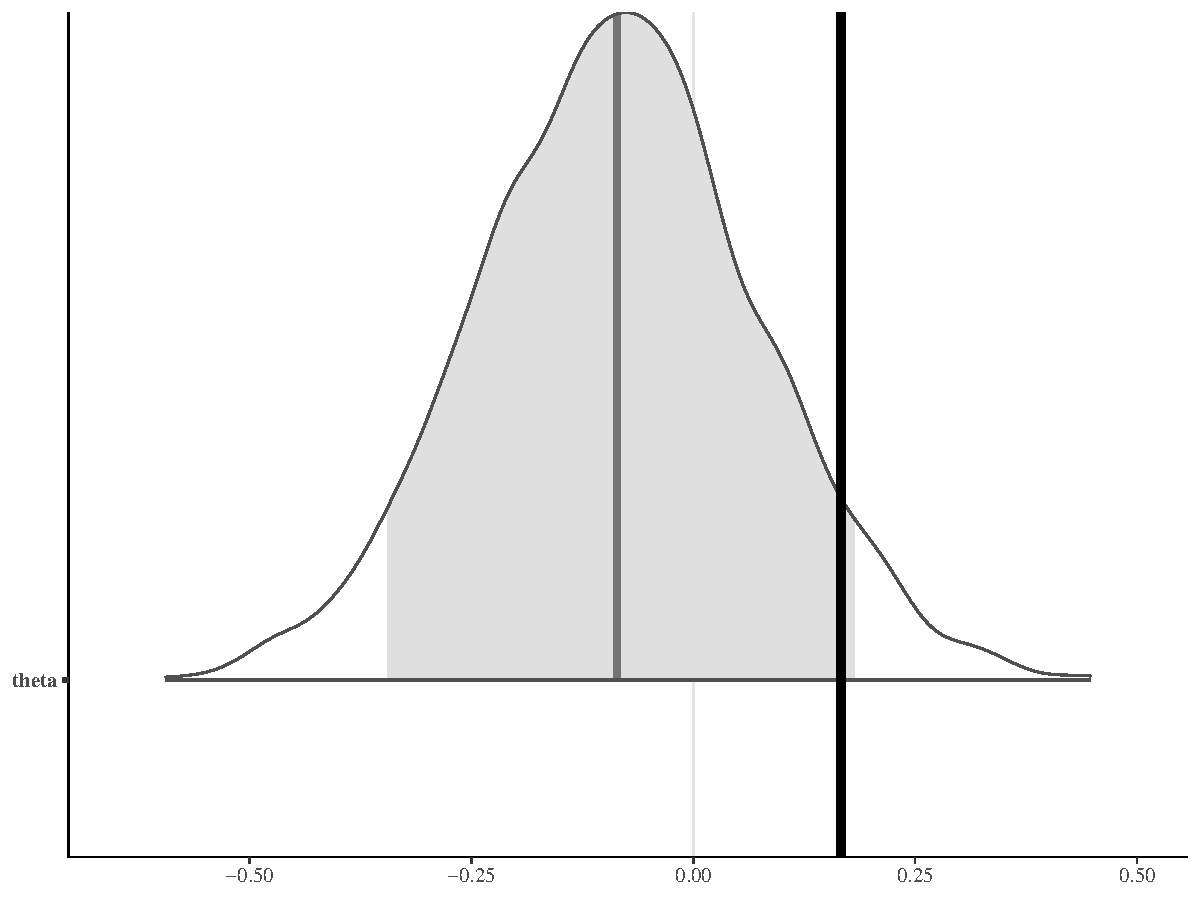
\includegraphics[width=0.65\textwidth]{theta-sim-res.pdf}
	\caption{Posterior estimates and known parameter value for the alliance hyperparameter $\theta$. The dark gray bar marks the posterior mean, while the shaded area captures the 90\% credible interval. The black line marks the known, ``true'' $\theta$ value, which falls within the 90\% interval.}
	\label{fig:theta-sim-res}
\end{figure}


\begin{figure}[htbp]
	\centering
		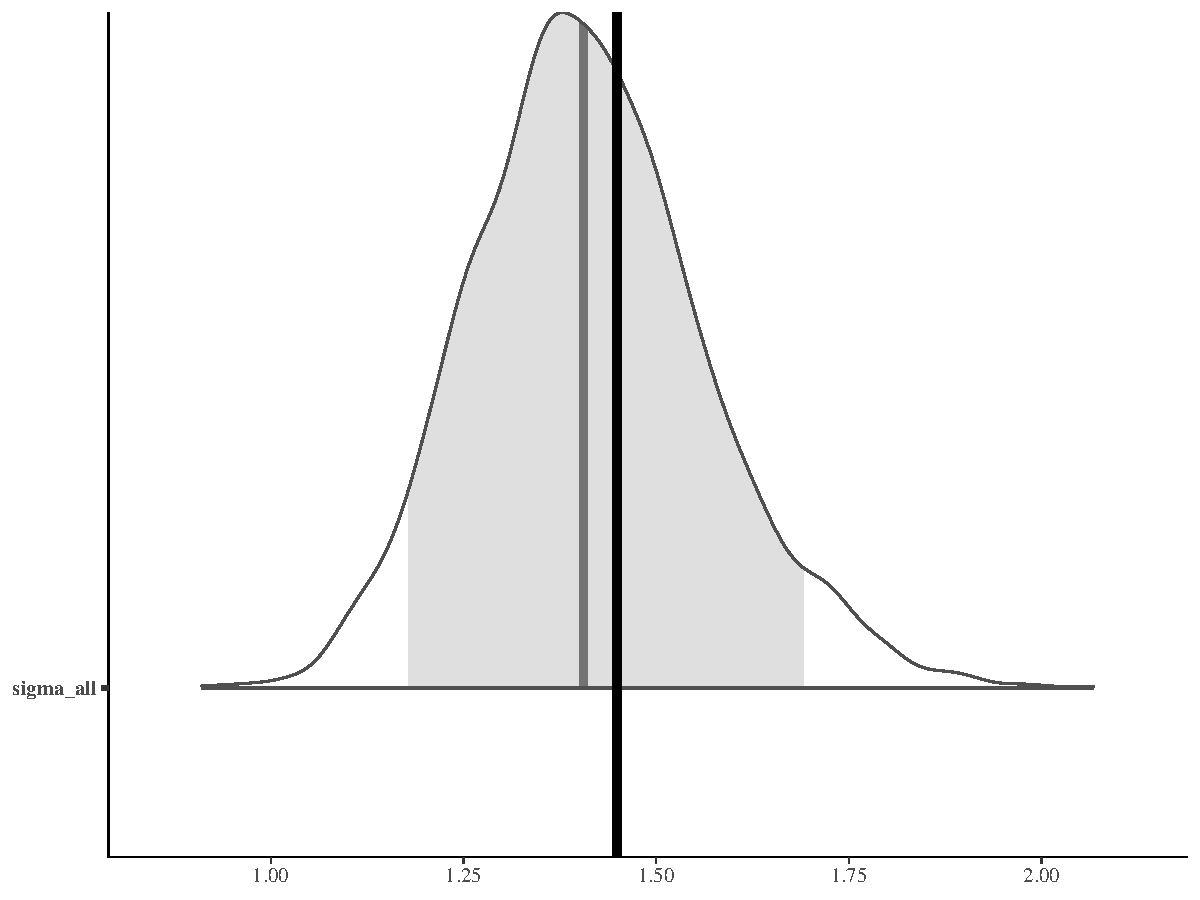
\includegraphics[width=0.65\textwidth]{sall-sim-res.pdf}
	\caption{Posterior estimates and known parameter value for the alliance hyperparameter $\sigma_{all}$. The dark gray bar marks the posterior mean, while the shaded area captures the 90\% credible interval. The black line marks the known, ``true'' $\sigma_{all}$ value, which falls within the 90\% interval.}
	\label{fig:sall-sim-res}
\end{figure}


Because graphical presentation of the 200 $\gamma$ parameters is more difficult, I calculated whether the credible interval contained the known parameter. 
91 of the 100 intervals include the ``true'' $\gamma$ value. 
Given the number of parameters and potential simulation variance, such accuracy is tolerable. 
Simulating data and recovering known parameters shows that the model estimates are reasonable approximations of the data-generating process. 


\subsection{Alternative Coding of Economic Size}


The values of -1 for small states and 1 for large states in the manuscript create coarse bins. 
This could mask differences within each category that affect inferences about economic weight and percentage changes in military spending within alliances. 
This section checks whether inferences are sensitive to an alternative coding of $\textbf{Z}$. 


To retain the same split of negative values for small states and positive values for large states, I subtracted one from economic weights that fell below the median in bilateral or multilateral alliances. 
This means that states with a small share of allied GDP have larger negative values than states with close to the median value. 
For example, a state with a 25\% of total allied GDP  in a bilateral alliance has a weight of -.75 with this variable, but a state with 49\% of allied GDP has a weight of -.51. 
Positive values remain the same.


Again, the public goods model would predict many positive $\gamma$ parameters, as these would reflect higher military spending for large states and lower military spending for small states. 
As \autoref{fig:alliance-coefs-year-w} shows, this is once again not the case. 
There are two alliances with a clearly positive $\gamma$ parameter. 
These are the OAS (ATOPID 3150) and an alliance between the United States and Thailand (ATOPID 3260). 
35 alliances have a positive posterior mean, as well. 

\begin{figure}[htbp]
	\centering
		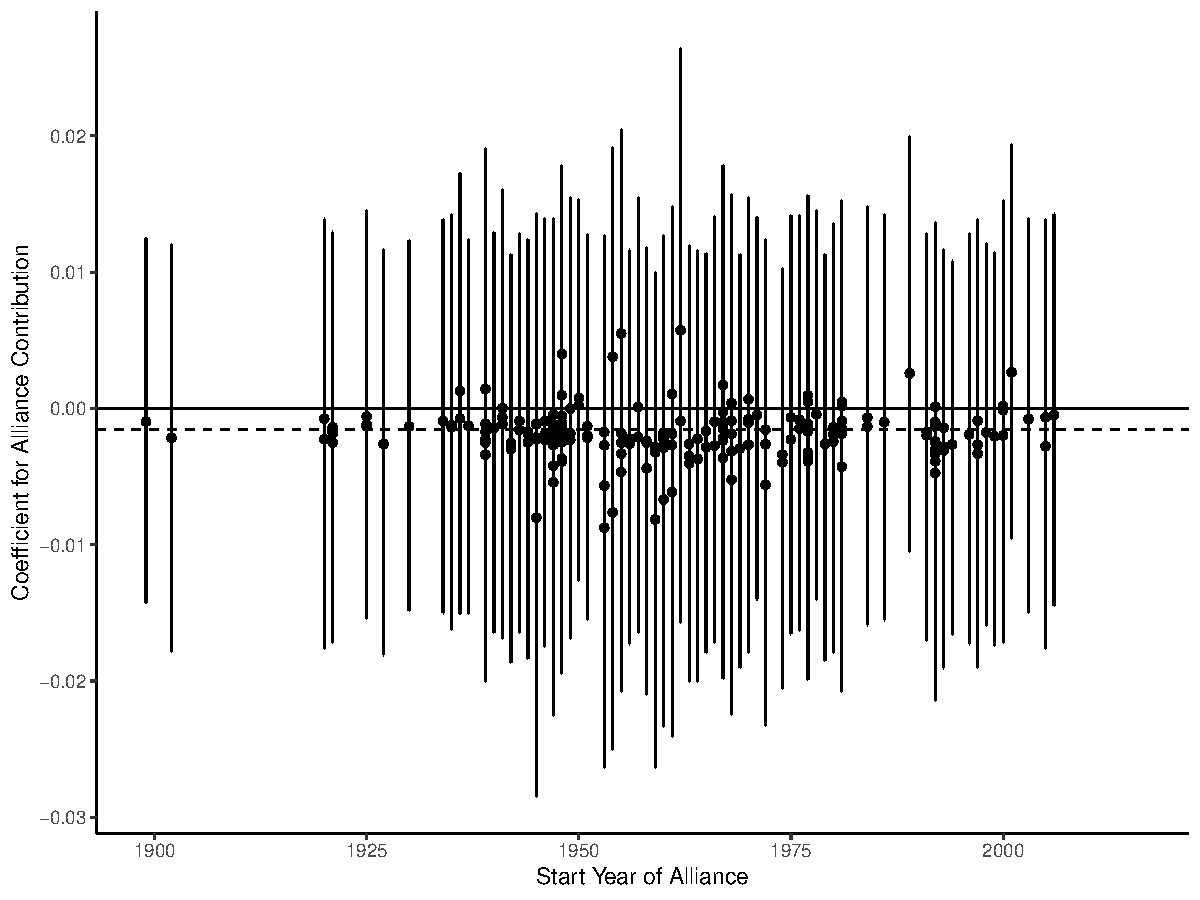
\includegraphics[width=0.95\textwidth]{alliance-coefs-year-w.pdf}
	\caption{Estimated $\gamma$ parameters from a model with negative and positive economic weights in the alliance membership matrix.}
	\label{fig:alliance-coefs-year-w}
\end{figure}

While this approach is somewhat better for the public goods model's predictions, it raises the same issues of generalizability. 
There are very few alliances with even limited evidence that economic weight leads to higher military spending. 



\section{Average Economic Weight and Military Spending}


The model I use in the paper estimates alliance-specific associations between economic weight and military spending. 
I also consider whether higher average economic weight across multiple alliances increases percentage changes in military spending. 
This section summarizes results from four models of the correlation between average economic weight and military spending. 
Following the recommendations of \citet{RaineyBaissa2018}, I use OLS and robust regression estimators with both transformed and unaltered military spending growth.  
I use an inverse hyperbolic sine to transform the outcome because this transformation includes positive, negative and zero values. 
Robust regression down weights unusual observations, which is important because the residuals of OLS estimators in this data are not normally distributed. 


The key independent variable is a state's average economic weight across all of its alliances. 
I also include measures of average alliance size and democracy \citep{DigiuseppePoast2016} as controls. 
Other controls are the same as the multilevel model.  


\autoref{tab:avg-weight-res} summarizes the results of these four estimation strategies. 
The robust regression coefficients for average economic weight are of small substantive magnitude and are statistically insignificant. 
The OLS estimates for average economic weight are larger, but the difference between these estimates and the robust regression suggests that unusual observations are the source of this difference. 


\begin{table}[!htbp] \centering 
  \caption{OLS and robust regression of the association between average economic weight in alliances and percentage changes in military expenditures from 1816 to 2007.} 
  \label{tab:avg-weight-res} 
\begin{tabular}{@{\extracolsep{5pt}}lcccc} 
\\[-1.8ex]\hline 
\hline \\[-1.8ex] 
 & \multicolumn{4}{c}{\textit{Dependent variable:}} \\ 
\cline{2-5} 
\\[-1.8ex] & \multicolumn{2}{c}{\% Change Milex.} & \multicolumn{2}{c}{IHS(\% Change Milex.)} \\ 
\\[-1.8ex] & \textit{Robust Reg.} & \textit{OLS} & \textit{OLS} & \textit{Robust} \\ 
\\[-1.8ex] & (1) & (2) & (3) & (4)\\ 
\hline \\[-1.8ex] 
 Average Economic Weight & $-$0.016 & 0.525 & 0.063 & $-$0.015 \\ 
  & (0.020) & (0.644) & (0.042) & (0.020) \\ 
  & & & & \\ 
 ln(GDP) & $-$0.119$^{***}$ & $-$6.384$^{***}$ & $-$0.468$^{***}$ & $-$0.118$^{***}$ \\ 
  & (0.046) & (1.462) & (0.096) & (0.046) \\ 
  & & & & \\ 
 Average Alliance Size & $-$0.0002 & $-$0.013 & 0.0002 & $-$0.0002 \\ 
  & (0.0004) & (0.012) & (0.001) & (0.0004) \\ 
  & & & & \\ 
 Average Allied Democracy & 0.001 & $-$0.032 & $-$0.001 & 0.001 \\ 
  & (0.001) & (0.025) & (0.002) & (0.001) \\ 
  & & & & \\ 
 International War & 0.109$^{***}$ & 0.570 & 0.248$^{***}$ & 0.108$^{***}$ \\ 
  & (0.012) & (0.381) & (0.025) & (0.012) \\ 
  & & & & \\ 
 Civil War Participant & $-$0.001 & 0.134 & 0.016 & $-$0.001 \\ 
  & (0.010) & (0.308) & (0.020) & (0.010) \\ 
  & & & & \\ 
 Regime Type & $-$0.001 & 0.039$^{**}$ & 0.001 & $-$0.001 \\ 
  & (0.001) & (0.019) & (0.001) & (0.001) \\ 
  & & & & \\ 
 External Threat & 0.057$^{***}$ & 1.195$^{**}$ & 0.117$^{***}$ & 0.057$^{***}$ \\ 
  & (0.015) & (0.472) & (0.031) & (0.015) \\ 
  & & & & \\ 
 Cold War & 0.047$^{***}$ & 0.387$^{**}$ & 0.039$^{***}$ & 0.046$^{***}$ \\ 
  & (0.006) & (0.179) & (0.012) & (0.006) \\ 
  & & & & \\ 
 Constant & 0.138$^{***}$ & 5.156$^{***}$ & 0.425$^{***}$ & 0.137$^{***}$ \\ 
  & (0.037) & (1.186) & (0.078) & (0.037) \\ 
\hline \\[-1.8ex] 
Observations & 5,409 & 5,409 & 5,409 & 5,409 \\ 
R$^{2}$ &  & 0.007 & 0.026 &  \\  
Residual Std. Error (df = 5399) & 0.157 & 6.034 & 0.397 & 0.156 \\ 
\hline 
\hline \\[-1.8ex] 
\textit{Note:}  & \multicolumn{4}{r}{$^{*}$p$<$0.1; $^{**}$p$<$0.05; $^{***}$p$<$0.01} \\ 
\end{tabular} 
\end{table} 

To asses the substantive impact of increasing a state's average economic weight in its alliances, I simulated the effect of moving average weight from the first quartile (0.05) to the third quartile (.40). 
Holding all other variables at their medians or modes, this increase in weight implies an expected percentage change in military spending of -0.005. 
The 90\% credible interval for this change ranges from -0.017 to 0.007, which implies that a substantively meaningful negative effect is more plausible. 



\newpage
\singlespace


\bibliography{../../../MasterBibliography} 





\end{document}
